\documentclass[11pt]{article}

\usepackage{fullpage}
\usepackage{graphicx}
\usepackage{parskip}

\begin{document}

\title{ARM Group 51 Checkpoint}
\author{Jamin Son, Lewen Oh, Xi Ting Hoh, Yuhan Wu}

\maketitle

\section{Group Organisation}

\subsection{Work Split and Coordination}

Our first priority was making sure that everyone in the group knew the fundamentals of the project. Understanding these parts was critical to understanding the project and so everyone worked together for this.

\begin{itemize}
        \item Background: What the emulator and assembler do and how the emulator and assembler fit within the context of process of compiling and running C code.
        \item Initial emulator high level overview.
        \item How the processor state was to be represented in C (Data registers and Memory).
\end{itemize}

Testing emulator code was also done by everyone. The remaining tasks were delegated as follows:

Lewen: Makefile; Binary File loader and output; Stitching together all the functions in emulator loop \newline
Yuhan: Data Processing Instruction (Registers); Single Data Transfer; Branch \newline
Xi Ting: Data Processing Instruction (Immediates)\newline
Jamin: Decoder; Git; Project Coordination

\subsection{Group Cohesion Evaluation}
Overall we are working well. Coordination of tasks was done with the goal of placing tasks to individual strengths and placing similar tasks to a single person. The benefit of this approach was evident as members could code instructions quicker as they became increasingly familiar with the problem and our implementation.

\textbf{Changes for later tasks:} Testing was an issue that we initially overlooked. Writing test's for each other's code was difficult due to the initial lack of consistent commenting thus resulting in delays. For future parts, commenting and writing easily comprehensible code will be one of our priorities.

\section{Implementation Strategies}
\subsection{Emulator Structure}
The processor state was implemented as follows:

\begin{figure}[ht]
        \centering
        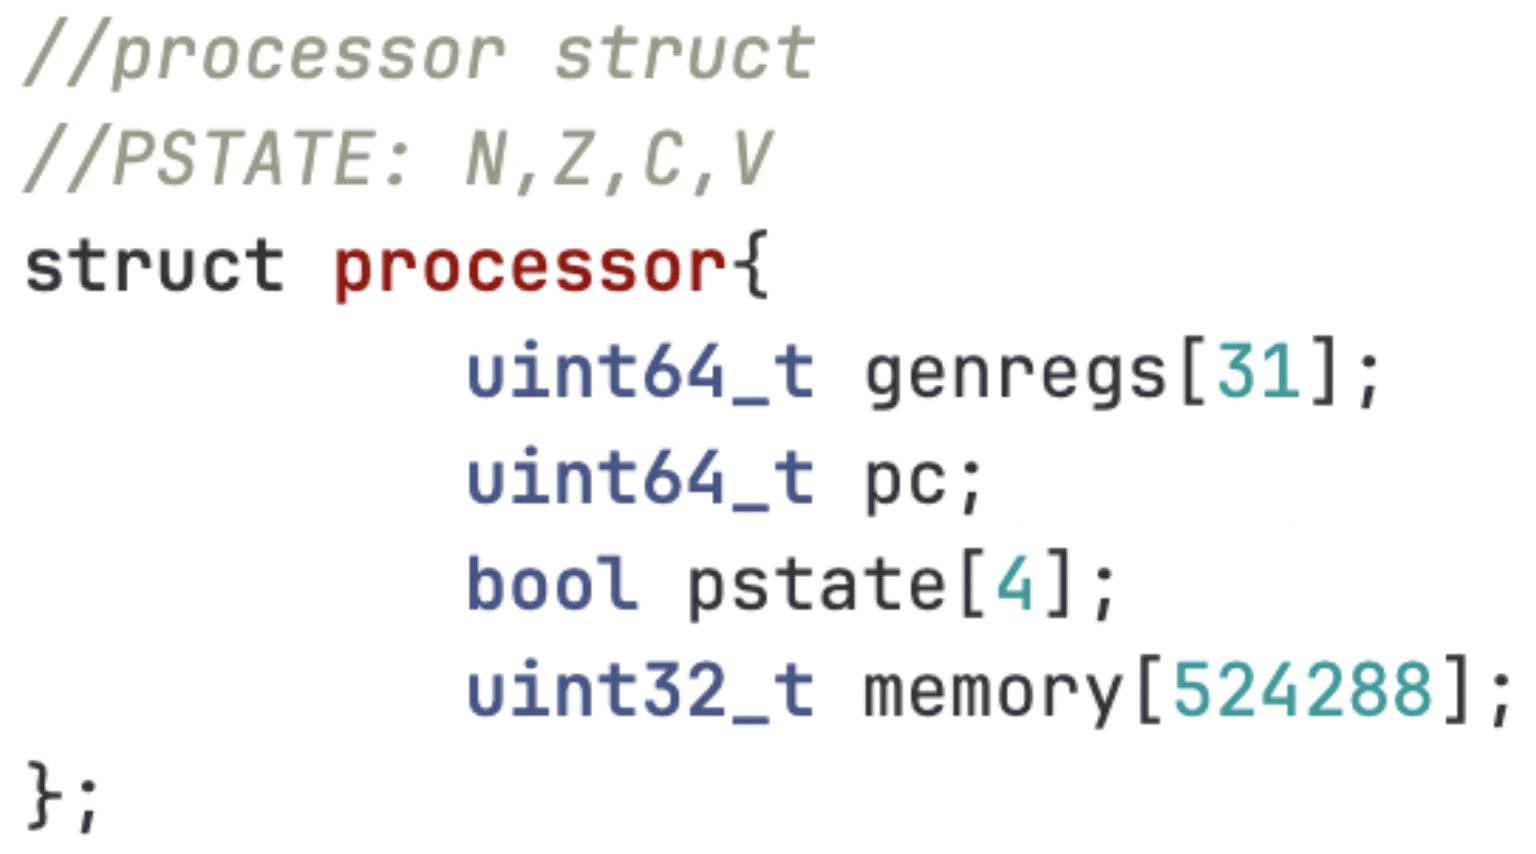
\includegraphics[width=0.3\linewidth]{struct}
\end{figure}

The emulator process consists of:
\begin{itemize}
        \item Reading the entire binary file into the memory array.
        \item Decoding each binary file.
        \item Executing the instruction based on the value of the decoder.
        \item Outputting the final processor state as required.
\end{itemize}

\textbf{Emulator Reuse in Assembler:} The emulator and assembler will bear general similarities, in that both will first understand the instruction then process it based on that information. Additionally, file loading will be achieved very similarly. We can thus expect file loading, the main assembler loop and, more generally, overall directory structure to be similar to its emulator counterparts. There will be further similarities in instruction decoding/encoding as both parts use equivalent instruction sets.

\subsection{Implementation Difficulties}
\textbf{Work Coordination:} One of the most difficult aspects has been coordinating coding between different people. Since functions and modules that would be interdependent are written it is hard to know how to structure your own programs. \textbf{Mitigation:} We tackled this issue by collectively planning out the emulator before and writing pseudocode for each function to allow us to decide function signatures as well as spot places where there is repeated code.

\textbf{Memory Implementation:} Deciding also how to represent memory in the program was difficult. It was initially unclear whether to implement it almost as a linked list - only adding entries (addresses and their values) as they were needed by the processor; or, whether to store the entire memory as a whole including its unused entries. We determined that it was possible to store the entire processor memory, but we had to reduce the required total size of the memory array ($2^{21}$) by a factor of 4 as the C would not compile otherwise. This was also done as each memory address would be 4 bytes long. We knew that this could cause complexity in implementation, and we tried to be careful about this. This still caused some grief later when testing load, store and branch instructions (for example when storing occurred into non-multiple of 4 addresses and the instructions spanned multiple bytes). \textbf{Mitigation:} We will be more cautious making such decisions for the assembler. However, we also learnt that not all errors can be predicted when planning, and the best way to mitigate these issues was creating program iterations quickly and to test often.

\end{document}
